\classheader{Lecture 3}
\setcounter{lecture}{3}

\begin{center}
	\Large \bf Set Functions
\end{center}

\vspace{0.25cm}

\begin{definition}
	$ c \subseteq \mathcal{P}\left(\Omega\right) $, $ \mu:  c \to \mathbb{R}_{+} \bigcup {+ \infty} $:
	\begin{enumerate}
		\item \label{def3.1.1} $ E \in c $, $ \mu $ continuous from below at $ E $, if $\forall {\left( {{E_n}} \right)_{n \geqslant 1}},\;{E_n} \in c,\;{E_n} \uparrow E\;\left( {{E_n} \subseteq {E_{n + 1}},\;\bigcup\limits_{n \geqslant 1} {{E_n} = E} } \right):$
		\begin{equation}
		\mu \left( {{E_n}} \right) \to \mu \left( E \right)
		\label{eq3.1}
		\end{equation}
		\item \label{def3.1.2}  $ E \in c $, $ \mu $ continuous from above at $ E $, if $\forall {\left( {{E_n}} \right)_{n \geqslant 1}},\;{E_n} \in c,\;{E_n} \downarrow E\;\left( {{E_{+1}} \subseteq {E_{n}},\;\bigcap\limits_{n \geqslant 1} {{E_n} = E} } \right),$ and $\exists {n_0},\;\mu \left( {{E_{{n_0}}}} \right) < \infty $:
		\begin{equation}
		\mu \left( {{E_n}} \right) \to \mu \left( E \right)
		\label{eq3.2}
		\end{equation}
	\end{enumerate}
\label{def3.1}
\end{definition}

\begin{remark}
	For a sequence $ E_{1},E_{2}, ... $ of sets, we put 
	\begin{equation}
	\lim \sup {E_i} = \bigcap\limits_{n = 1}^\infty  {\left( {\bigcup\limits_{i = n}^\infty  {{E_i}} } \right)} ,\lim \inf {E_i} = \bigcup\limits_{n = 1}^\infty  {\left( {\bigcap\limits_{i = n}^\infty  {{E_i}} } \right)} 
	\end{equation}
	and if $\left\{ {{E_i}} \right\}$ is such that ${\lim \sup E = \lim \inf {E_i}}$ we say that the sequence converges to the set 
	\begin{equation}
	{E = \lim \sup E = \lim \inf {E_i}}
	\end{equation}
	\label{rmk3.1}
\end{remark}

\begin{remark}
	\ref{def3.1.2} need $\exists {n_0},\;\mu \left( {{E_{{n_0}}}} \right) < \infty $, if not: \
	\begin{equation}
	{E_n} = \left[ {n, + \infty } \right),\;\mu \left( {{E_n}} \right) =  + \infty ,\;{E_n} \downarrow \emptyset ,\;\lambda \left( \emptyset  \right) = 0
	\label{eq3.3}
	\end{equation}
	\label{rmk3.2}
\end{remark}

\begin{lemma}
	$ a \subseteq \mathcal{P}\left(\Omega\right) $, algebra; $\mu :\;a \to {\mathbb{R}_ + } \cup \left\{ { + \infty } \right\}$, additive;
	\begin{enumerate}
		\item \label{lem3.1.1} $ \mu $ is $ \sigma $-additive $ \Rightarrow $ $ \mu  $ continuous at E, $ \forall E \in a $
		\item \label{lem3.1.2} $ \mu $ is continuous from below $ \Rightarrow $ $ \mu  $  is $ \sigma $-additive 
		\item \label{lem3.1.3} $ \mu $ is continuous from above at $ \emptyset \&  $ $ \mu $ is finite $ \Rightarrow $ $ \sigma $-additive 
	\end{enumerate}
\label{lem3.1}
\end{lemma}

\begin{proof}
	\text{}
	\begin{enumerate}
		\item \text{}
		
		(i) $ \mu  $ is $ \sigma $-additive $ \Rightarrow $ $ \mu $ conti. from below at $  E \in a. $
		\begin{figure}[!htb]
			\centering
			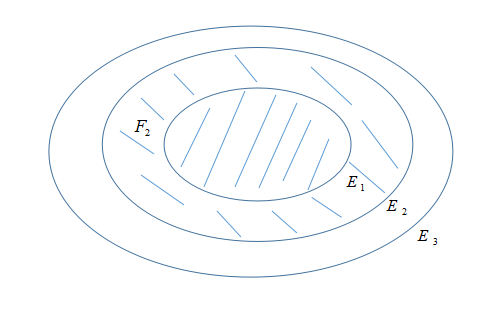
\includegraphics[width=0.3\linewidth,height=0.2\linewidth]{fig31.png}
			\label{fig31}
			%\caption{ illustration for $ 3 $}
		\end{figure}
	    $ E \in a, {E_n} \uparrow E,\;{E_n} \in a$:
	    \begin{equation}
	    \begin{split}
	    {F_1} & = {E_1} \\
	    {F_2} & = {E_2}\backslash {E_1}\\
	     \vdots \ \  & = \ \  \vdots  \\
	    {F_n} & = {E_n}\backslash {E_{n - 1}}
	    \end{split}
	    \label{eq3.4}
	    \end{equation}
	    and we can get that
	    \begin{equation}
	    {F_j} \cap {F_k} = \emptyset ,\quad \sum\limits_{k = 1}^n {{F_k}}  = {E_n}, \quad \bigcup\limits_{n \geqslant 1} {{E_n}}  = \bigcup\limits_{n \geqslant 1} {{F_n}} 
	    \label{eq3.5}
	    \end{equation}
	    so 
	    \begin{equation}
	    \mu \left( E \right) = \sum\limits_{k \geqslant 1} {\mu \left( {{F_k}} \right)}  = \mathop {\lim }\limits_{n \to \infty } \sum\limits_{k = 1}^n {\mu \left( {{F_k}} \right)}  = \mathop {\lim }\limits_{n \to \infty } \mu \left( {{E_n}} \right)
	    \label{eq3.6}
	    \end{equation}
		(ii) $ \mu $ cont. from above $ E \in a, {E_n} \in a,{E_n} \downarrow E,\mu \left( {{E_{{n_0}}}} \right) < \infty  \Rightarrow \mu \left( {{E_n}} \right) \downarrow \mu \left( E \right)$
		\begin{figure}[!htb]
			\centering
			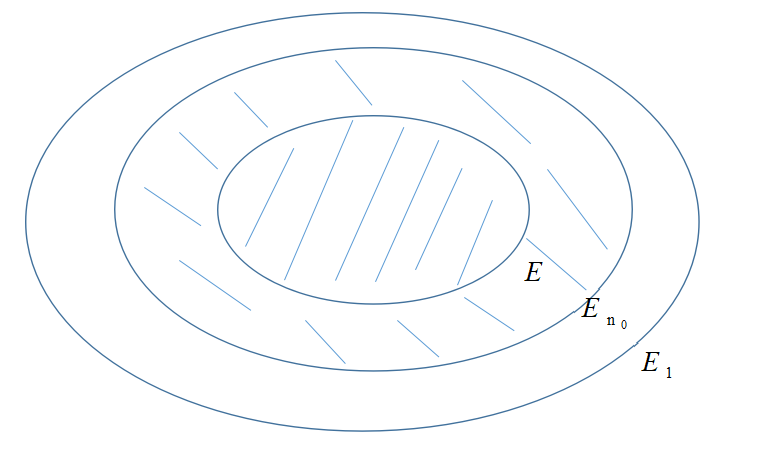
\includegraphics[width=0.3\linewidth,height=0.2\linewidth]{fig32.png}
			\label{fig32}
			%\caption{ illustration for $ 3 $}
		\end{figure}
		\begin{equation}
		\begin{split}
		{G_1} & = {E_{{n_0}}}\backslash {E_{{n_0} + 1}}\\
		{G_2} & = {E_{{n_0}}}\backslash {E_{{n_0} + 2}} \\
		\vdots \quad & = \quad \vdots\\
		{G_k} & = {E_{{n_0}}}\backslash {E_{{n_0} + k}}
		\end{split}
		\label{eq3.7}
		\end{equation}
		then ${G_k} \uparrow {E_{{n_0}}}\backslash {E}, {G_k} \in a \Rightarrow \mu \left( {{G_k}} \right) \uparrow \mu \left( {{E_{{n_0}}}\backslash E} \right)$, so
		
		\begin{equation}
		\begin{split}
		\mu \left( {{E_{{n_0}}}\backslash E} \right) & = \mathop {\lim }\limits_{n \to \infty } \mu \left( {{E_{{n_0}}}\backslash {E_{{n_0} + k}}} \right)\\
		\mu \left( {{E_{{n_0}}}\backslash E} \right) & = \mu \left( {{E_{{n_0}}}} \right) - \mu \left( E \right)\\
		\mu \left( {{E_{{n_0}}}} \right) - \mu \left( E \right) & = \mathop {\lim }\limits_{k \to \infty } \left( {\mu \left( {{E_{{n_0}}}} \right) - \mu \left( {{E_{{n_0} + k}}} \right)} \right)
		\end{split}
		\end{equation}
		\label{eq3.8}
		\item $ \mu $ cont. below, $E = \sum\limits_{k \geqslant 1} {{E_k}} ,\;E,{E_k} \in a$.
		
		Obs.
		\begin{equation}
		\sum\limits_{k = 1}^n {{E_k}}  \subseteq E \stackrel{additive}{\Rightarrow} \left\{ \begin{matrix} 
		\mu \left( {\sum\limits_{k = 1}^n {{E_k}} } \right) \leqslant \mu \left( E \right) \hfill \cr 
		\sum\limits_{k = 1}^n {\mu \left( {{E_k}} \right) \leqslant \mu \left( E \right)}  \hfill \cr 
		\end{matrix}  \right.
		\label{eq3.9}
		\end{equation}
		then
		\begin{equation}
		\sum\limits_{k \geqslant 1} {\mu \left( {{E_k}} \right)}  \leqslant \mu \left( E \right)
		\label{eq3.10}
		\end{equation}
		${F_n} = \sum\limits_{k = 1}^n {{E_k}}  \in a,\;{F_n} \uparrow E$, 
		\begin{equation}
		\sum\limits_{k = 1}^n {\mu \left( {{E_k}} \right)}  = \mu \left( {{F_n}} \right) \uparrow \mu \left( E \right) \Rightarrow \sum\limits_{k \geqslant 1} {\mu \left( {{E_k}} \right)}  = \mu \left( E \right)
		\label{eq3.11}
		\end{equation}
		\item $ \mu $ cont. at $ \emptyset $, $ \mu\left(\Omega\right) < \infty $, $ E,E_{k} \in a, E = \sum\limits_{k \geqslant 1} {{E_k}}. $ 
		\begin{equation}
		{F_n} = \sum\limits_{k \geqslant m} {{E_k}}  \in a\;\left( {E\backslash \sum\limits_{j = 1}^{n - 1} {{E_j}} } \right)
		\label{eq3.12}
		\end{equation}
		${F_n} \downarrow \emptyset ,\mu \left( {{F_1}} \right) < \infty ,\;\mu \left( {{F_n}} \right) \to 0$
		\begin{equation}
		\begin{split}
		\mu \left( E \right) & = \mu \left( {\sum\limits_{k = 1}^n {{E_k} \cup \sum\limits_{k > n} {{E_k}} } } \right)\\
							 & =  \underbrace {\mu \sum\limits_{k = 1}^n {{E_k}  } }_{ \to \sum\limits_{k \geqslant 1} {\mu \left( {{E_n}} \right)} } \ + \ \underbrace {\mu \sum\limits_{k > n} {{E_k}} }_{ \to 0}\\
							 & \to \sum\limits_{k \geqslant 1} {\mu \left( {{E_n}} \right)} 
		\end{split}
		\end{equation}
		\label{eq3.13}
	\end{enumerate}
\end{proof}

\begin{remark}
	Suppose ${E_\alpha },\;\alpha  \in I$ is a class of subsets of $ X $, and $ E_{i} $ is one set of the class, then
	\begin{enumerate}
		\item $\bigcap\limits_{\alpha  \in I} {{E_\alpha } \subseteq {E_i}}  \subseteq \bigcup\limits_{\alpha  \in I} {{E_\alpha }} $
		\item \label{rmk332}$ X - \bigcup\limits_{\alpha  \in I} {{E_\alpha }}  = \bigcap\limits_{\alpha  \in I} {\left( {X - {E_\alpha }} \right)} $
		\item \label{rmk333}$ X - \bigcap\limits_{\alpha  \in I} {{E_\alpha }}  = \bigcup\limits_{\alpha  \in I} {\left( {X - {E_\alpha }} \right)} $
	\end{enumerate}
	\label{rmk3.3}
\end{remark}

\begin{proof}
	\text{}
	\begin{enumerate}
		\item This is immediate from the definition.
		\item Suppose $ x \in  X - \bigcup\limits_{\alpha  \in I} {{E_\alpha }} $ then $ x \in X $  and x is not in $ \bigcup\limits_{\alpha  \in I} {{E_\alpha }} $, that is $ x $ is not in any $  E_{\alpha} $, $ \alpha \in I $ so that $ x \in X - E_{\alpha} $ for every $ \alpha \in I $, and  $ x \in \bigcap\limits_{\alpha  \in I} {\left( {X - {E_\alpha }} \right)}. $ Conversely if  $ x \in \bigcap\limits_{\alpha  \in I} {\left( {X - {E_\alpha }} \right)}$, then for every $ \alpha \in I $, $ x $ is in $ X $ but not in $ E_{\alpha} $, so $ x  \in X$ but $ x $  is not in $\bigcup\limits_{\alpha  \in I} {{E_\alpha }} $, that is $x \in \bigcup\limits_{\alpha  \in I} {\left( {X - {E_\alpha }} \right)} $.
		\item Similar to 2
	\end{enumerate}	
Remark \ref{rmk3.3} (\ref{rmk332}) and (\ref{rmk333}) are also called as de Morgan's Law.	
\end{proof}

\begin{example}
	$\left( {0,1} \right),\left( {a,b} \right],0 \leqslant a < b < 1$
	\begin{equation}
	\mu \left( {a,b} \right] = \left\{ {\begin{matrix}
		{b - a,}  \\ 
		{ + \infty ,}  \\ 
		
		\end{matrix} } \right.\;\begin{matrix}
	{a > 0}  \\ 
	{a = 0}  \\ 
	
	\end{matrix} 
	\label{eq3.16}
	\end{equation}
	$ \mu  $ is additive but NOT $ \sigma $-additive
\end{example}

\begin{proof}
	${E_n} \downarrow \emptyset ,\;\mu \left( {{E_{{n_0}}}} \right) < \infty ,\;{E_n} = \left( {{a_{n,1}},{b_{n,1}}} \right] \cup  \cdots  \cup \left( {{a_{n,{k_n}}},{b_{n,{k_n}}}} \right],{a_{n,j}} < {a_{n,j + 1}}.$ 
	
	$\left\{ {\begin{matrix}
		{{a_{n,1}} = 0,}  \\ 
		{{a_{{n_0}}} > 0,}  \\ 
		
		\end{matrix} } \right.\begin{matrix}
	{\forall n}  \\ 
	{some\;{n_0}}  \\ 
	
	\end{matrix} $
\end{proof}

\begin{theorem}[Extension]
	$ f \subseteq \mathcal{P}\left(\Omega\right) $ semi-algebra, $ \mu  :f \to {\mathbb{R}_ + } \cup \left\{ \infty  \right\}$ {\color{blue}$ \sigma $-}additive, then $ \exists \nu: $ 
	\begin{equation}
	\nu :a\left( f \right) \to {\mathbb{R}_ + } \cup \left\{ \infty  \right\}
	\end{equation}
	such that:
	\begin{enumerate}
		\item $ \nu $ {\color{blue}$ \sigma $-}additive
		\item $\nu \left( A \right) = \mu \left( A \right),\;\forall A \in f$
		\item $ \mu_{1},\mu_{2}, a\left(f\right) \to \mathbb{R}_{+} \bigcup \left\{ { + \infty } \right\}, $ then $ {\mu _1}\left( A \right) = {\mu _2}\left( A \right),\forall A \in s \Rightarrow {\mu _1}\left( E \right) = {\mu _2}\left( E \right),\forall E \in a\left( f \right) $	
	\end{enumerate}
\label{thm3.1}
\end{theorem}
\begin{proof}
	$ A \in a(f) \Rightarrow A = \sum\limits_{j = 1}^n {{E_j}} ,\;{E_j} \in f $ by Lemma  \ref{lma2.1}.
	\begin{equation}
	\nu \left( A \right) \stackrel{add}{=} \sum\limits_{j = 1}^n {\nu \left( {{E_j}} \right)}  \stackrel{ext}{=} \sum\limits_{j = 1}^n {\mu \left( {{E_j}} \right)} 
	\end{equation}
	we define that
	\begin{equation}
	\nu \left( A \right) = \sum\limits_{j = 1}^n {\mu \left( {{E_j}} \right)} 
	\label{eq3.19}
	\end{equation}
	we want to show that $\nu \left( A \right) = \sum\limits_{j = 1}^n {\mu \left( {{E_j}} \right)} $ is well-defined:
	\begin{enumerate}
		\item $ \nu $ is unique
		\begin{equation}
		\begin{split}
		A & = \sum\limits_{j = 1}^n {{E_j}} ,\;{E_j} \in f\\
		  & = \sum\limits_{k = 1}^m {{F_k}} ,\;{F_k} \in f
		\end{split}
		\end{equation}
		then we will prove that 
		\begin{equation}
		\begin{split}
		\nu \left( A \right) & = \sum\limits_{j = 1}^n {\mu \left( {{E_j}} \right)} \\
							 & = \sum\limits_{k = 1}^m {\mu \left( {{F_k}} \right)} 
		\end{split}
		\end{equation}
		\begin{equation}
		\because {E_j} \subseteq A = \sum\limits_{k = 1}^m {F{}_k}  \Rightarrow {E_j} = {E_j} \cap \left( {\sum\limits_{k = 1}^m {F{}_k} } \right) = \sum\limits_{k = 1}^m {\underbrace {\left( {{E_j} \cap {F_k}} \right)}_{ \in f}} 
		\end{equation}
		\begin{equation}
		\therefore \mu \left( {{E_j}} \right) = \mu \left( {\sum\limits_{k = 1}^m {\left( {{E_j} \cap {F_k}} \right)} } \right)
		\end{equation}
		then 
		\begin{equation}
		\nu \left( A \right) = \sum\limits_{j = 1}^n {\mu \left( {{E_j}} \right)}  = \sum\limits_{j = 1}^n {\sum\limits_{k = 1}^m {\mu \left( {{E_j} \cap {F_k}} \right) = } } \sum\limits_{k = 1}^m {\mu \left( {{F_k}} \right)} 
		\end{equation}
		\item $ \nu $ is an additive, $\nu \left( A \right) = \sum\limits_{j = 1}^n {\mu \left( {{E_j}} \right)}  $
		
		Assume that
		\begin{equation}
		\left\{ {\begin{matrix}
			{A = \sum\limits_{j = 1}^n {{E_j}} ,\;{E_j} \in f}  \\ 
			{B = \sum\limits_{k = 1}^m {{F_k}} ,\;{F_k} \in f}  \\ 
			\end{matrix} } \right.,A \cap B = \emptyset 
		\end{equation}
		
		We will show that 
		\begin{equation}
		\nu \left( {A \cup B} \right) = \nu \left( A \right) + \nu \left( B \right)
		\end{equation}
		
		\begin{equation}
		\because A \cup B = \sum\limits_{j = 1}^n {{E_j}}  + \sum\limits_{k = 1}^m {{F_k}} 
		\end{equation}
		therefore 
		\begin{equation}
		\begin{split}
		\nu \left( {A \cup B} \right) & = \mu \left( {\sum\limits_{j = 1}^n {{E_j}}  + \sum\limits_{k = 1}^m {{F_k}} } \right)\\
									  & = \sum\limits_{j = 1}^n {\mu \left( {{E_j}} \right) + \sum\limits_{k = 1}^m {\mu \left( {{F_k}} \right)} } \\
									  & = \nu \left( A \right) + \nu \left( B \right)
		\end{split}
		\end{equation}
		\item $\nu \left( A \right) = \mu \left( A \right),\;A \in f$ by Eq \ref{eq3.19}
		
		\item $ \nu $ is uniqueness, we want to show that:
		
		Suppose that ${\mu _1},{\mu _2}:\;\;a\left( f \right) \to {R_ + } \cup \left\{ { + \infty } \right\},\forall A\; \in f,{\mu _1},{\mu _2}\;additive$,  then
		\begin{equation}
		{\mu _1}\left( A \right) = {\mu _2}\left( A \right) \Rightarrow {\mu _1}\left( B \right) = {\mu _2}\left( B \right),\;\forall B \in a\left( f \right)
		\end{equation}
		
		$ \because B \in a\left(f\right), \therefore B = \sum\limits_{j = 1}^n {{\mu _1}\left( {{E_j}} \right)} ,\;{E_j} \in f $ 
		\begin{equation}
		{\mu _1}\left( B \right) = \sum\limits_{j = 1}^n {{\mu _1}\left( {{E_j}} \right)}  = \sum\limits_{j = 1}^n {{\mu _2}\left( {{E_j}} \right)}  = {\mu _2}\left( B \right)
		\end{equation}
	\end{enumerate}

    Now we proof the extension of {\color{blue} $ \sigma $}-additive, ie: $ \mu-\sigma $ additive, $ f $ semi-algebra, $ \nu -\sigma $ additive, $ a(f) $ is a algebra generated by $ f. $ we want to show that
    \begin{equation}
    A = \sum\limits_{j \geqslant 1} {{A_j}} ,\;A,{A_j} \in a\left( f \right) \Rightarrow \nu \left( A \right) = \sum\limits_{j \geqslant 1} {\nu \left( {{A_j}} \right)} 
    \end{equation}
    
    by representation of an algebra:
    \begin{equation}
    A = \sum\limits_{j = 1}^m {{E_j}} ,{E_j} \in f;\;\;\;\;{A_k} = \sum\limits_{l = 1}^{{m_k}} {{E_{k,l}}} ,{E_{k,l}} \in f
    \end{equation}
    by Eq \ref{eq3.19}:
    \begin{equation}
    \nu \left( A \right) = \sum\limits_{j = 1}^m {\nu \left( {{E_j}} \right)} ,\;\;\;\nu \left( {{A_k}} \right) = \sum\limits_{l = 1}^{{m_k}} {\nu \left( {{E_{k,l}}} \right)} 
    \end{equation}
    
   \begin{equation}
   \because {E_j} = {E_j} \cap A = {E_j} \cap \left( {\sum\limits_{k \geqslant 1} {{A_k}} } \right) = {E_j} \cap \left( {\sum\limits_{k \geqslant 1} {\sum\limits_{l = 1}^{{m_k}} {{E_{k,l}}} } } \right) = \sum\limits_{k \geqslant 1} {\sum\limits_{l = 1}^{{m_k}} {\left( {{E_j} \cap {E_{k,l}}} \right)} } 
   \end{equation}
   
   therefore
   
   \begin{equation}
   \begin{split}
   \nu \left( A \right) & = \sum\limits_{j = 1}^n {\mu \left( {{E_j}} \right)}\\
   						& = \sum\limits_{j = 1}^n {\sum\limits_{k \geqslant 1} {\sum\limits_{l = 1}^{{m_k}} {\mu \left( {{E_j} \cap {E_{k,l}}} \right)} } } \\
   						& = \sum\limits_{k \geqslant 1} {\underbrace {\sum\limits_{l = 1}^{{m_k}} {\mu \left( {{E_{k,l}}} \right)} }_{ \subseteq {A_k}}} 
   \end{split}
   \label{eq3.35}
   \end{equation}
   
   Eq \ref{eq3.35} holds because:
   \begin{equation}
  {E_{k,l}} = {E_{k,l}} \cap A = \sum\limits_{j = 1}^n {\left( {{E_{k,l}} \cap {E_j}} \right)} 
  \label{eq3.36}
   \end{equation}
   
   and
   \begin{equation}
   \mu \left( {{E_{k,l}}} \right) = \sum\limits_{j = 1}^n {\mu \left( {{E_{k,l}} \cap {E_j}} \right)} 
   \end{equation}
   
   so we can get that
   \begin{equation}
   \nu \left( A \right) = \sum\limits_{k \geqslant 1} {\nu \left( {{A_k}} \right)}
   \label{eq3.38} 
   \end{equation}
   
\end{proof}